\begin{abstract}
Language is the
\end{abstract}

\section{Introduction}
Effective communication across languages is crucial in today's globalized world. Machine translation (MT) bridges language barriers by automatically converting text from one language to another. Traditional MT approaches often relied on complex linguistic rules and struggled to capture the nuances of natural language. Neural machine translation (NMT) offers a powerful alternative which leverages deep learning techniques to translate languages directly, achieving higher accuracy and fluency compared to traditional methods. Developing such model is not easy due to the data requirement and computational cost, so to have an insight through them, we will develop some simplistic model from scratch and fine-tuning existing model to translate engineering assessments from English to Afrikaans, with a small dataset. For that purpose we present briefly the basic architecture used in NMT in section \ref{nmt}.  Then, the   section \ref{mth} focus on the methodology and finally present and discuss the result of our experimentation in the section \ref{res}.

\section{Neural Machine Translation}\label{nmt}
Translation task consist into converting a text $\mbf{x}=x_{1:T}$ from a language $A$ into a text $\mbf{y}=y_{1:S}$ of a language $B$, that have the same meaning and sense.

Compared to human, computer does not understand text and even words. But, with the appropriate modelling and tools it can perform such tasks. For Neural Machine Translation (NMT), it assigns a probability  $P_{\mbf{\theta}}(y|x)$ for any possible translation $y$ of $x$ then choose the the one with the highest probability. In that case the probability of the whole translation is given by :
\begin{equation}
P(\mbf{y}|\mbf{x})=\prod_{t=1}^S P_{\mbf{\theta}}(y_t|y_{1:t-1}, \mbf{x})
\end{equation}
where $\mbf{\theta}$ is the model parameters.
To implement this model, as indicated by the name NMT use neural network, specifically Encoder-Decoder architecture, illustrated in Figure \ref{fig:enc-dec} and \ref{fig:seq2seq}. In the Encoder part, the input are compressed into a smaller representation, which is feed into the Decoder part to produce an input with a specific target.
\begin{figure}[H]
	\centering
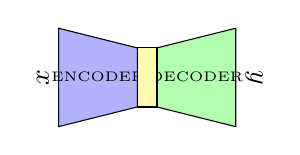
\begin{tikzpicture}
	\draw[fill=blue!30]  (0,0) -- (1, -0.25) -- (1, -1) -- (0,-1.25) -- cycle node[midway, left] {\rotatebox{90}{$\mbf{x}$}};
	\node[font=\tiny](enc) at (0.5, -0.62) {ENCODER};


	\draw[fill=green!30]  (1.25,-0.25) -- (2.25, 0) -- (2.25, -1.25) node[midway, right] {\rotatebox{-90}{$\mbf{y}$}}-- (1.25,-1) -- cycle;
	\node[font=\tiny](enc) at (1.75, -0.62) {DECODER};
	\draw[fill=yellow!30] (1, -.25) rectangle (1.25, -1);

\end{tikzpicture}
\caption{Illustration of an encoder-decoder architecture}
\label{fig:enc-dec}
\end{figure}
Treating, text data as a sequence, we use Recurrent Neural Networks (RNNs, Figure \ref{fig:rnn}), which predict a single word at a time, and the model is often call seq2seq (sequence-to-sequence) model. The particularity, of Recurrent neuron is to depend on its previous outputs or states.
\begin{figure}[H]
	\centering
\begin{subfigure}{0.2\linewidth}
\scalebox{0.75}{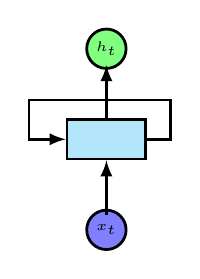
\begin{tikzpicture}
		\draw[line width=1pt, fill=blue!50] (0,-1.15) circle (0.25);
		\draw[line width=1pt, fill=green!50] (0,1.15) circle (0.25);
		\node[font=\tiny] (x) at (0, -1.15) {$\mbf{x_t}$};
		\node[font=\tiny] (h) at(0, 1.15) {$\mbf{h_t}$};
		\node[draw, rectangle, minimum height=0.5cm, minimum width=1cm, line width=1pt, fill=cyan!30] (a) at (0,0) {};
		\draw[->,>=latex, line width=1pt] (x.north)--(a);
		\draw[->,>=latex, line width=1pt] (a)--(h);
		\draw[line width=1pt,->, >=latex] (a.east) --++(0.3, 0) --++(0, 0.5) --++(-1.8,0) --++(0, -0.5) -- (a.west);
\end{tikzpicture}}
\caption{An RNN}
\label{fig:rnn}
\end{subfigure}\begin{subfigure}{0.8\linewidth}
\scalebox{0.75}{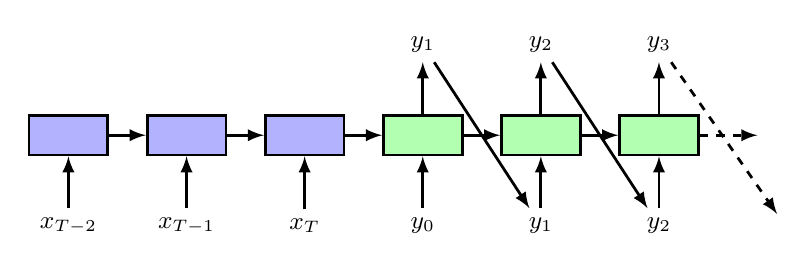
\begin{tikzpicture}
\begin{scope}
	\node[font=\small] (x) at (0, -1.15) {$\mbf{x_{T-2}}$};
	\node[draw, rectangle, minimum height=0.5cm, minimum width=1cm, line width=1pt, fill=blue!30] (e1) at (0,0) {};
	\draw[->,>=latex, line width=1pt] (x)--(e1);
\end{scope}
\begin{scope}[xshift=1.5cm]
	\node[font=\small] (x) at (0, -1.15) {$\mbf{x_{T-1}}$};
	\node[draw, rectangle, minimum height=0.5cm, minimum width=1cm, line width=1pt, fill=blue!30] (e2) at (0,0) {};
	\draw[->,>=latex, line width=1pt] (x)--(e2);
\end{scope}
\begin{scope}[xshift=3cm]
	\node[font=\small] (x) at (0, -1.15) {$\mbf{x_T}$};
	\node[draw, rectangle, minimum height=0.5cm, minimum width=1cm, line width=1pt, fill=blue!30] (e3) at (0,0) {};
	\draw[->,>=latex, line width=1pt] (x)--(e3);
\end{scope}

%%%%%%%%%%%%%%%%%%%%%%%%%%%
\begin{scope}[xshift=4.5cm]
	\node[font=\small] (x1) at (0, -1.15) {$\mbf{y_0}$};
	\node[font=\small] (y1) at (0, 1.15) {$\mbf{y_1}$};
	\node[draw, rectangle, minimum height=0.5cm, minimum width=1cm, line width=1pt, fill=green!30] (d1) at (0,0) {};
	\draw[->,>=latex, line width=1pt] (x1)--(d1);
	\draw[->,>=latex, line width=1pt] (d1)--(y1);
\end{scope}
\begin{scope}[xshift=6cm]
	\node[font=\small] (x2) at (0, -1.15) {$\mbf{y_1}$};
	\node[font=\small] (y2) at (0, 1.15) {$\mbf{y_2}$};
	\node[draw, rectangle, minimum height=0.5cm, minimum width=1cm, line width=1pt, fill=green!30] (d2) at (0,0) {};
	\draw[->,>=latex, line width=1pt] (x2)--(d2);
	\draw[->,>=latex, line width=1pt] (d2)--(y2);
\end{scope}
\begin{scope}[xshift=7.5cm]
	\node[font=\small] (x3) at (0, -1.15) {$\mbf{y_2}$};
	\node[font=\small] (y3) at (0, 1.15) {$\mbf{y_3}$};
	\node[draw, rectangle, minimum height=0.5cm, minimum width=1cm, line width=1pt, fill=green!30] (d3) at (0,0) {};
	\draw[->,>=latex, line width=1pt] (x3)--(d3);
	\draw[->,>=latex, line width=1pt] (d3)--(y3);
\end{scope}


\draw[->,>=latex, line width=1pt] (e1)--(e2);
\draw[->,>=latex, line width=1pt] (e2)--(e3);
\draw[->,>=latex, line width=1pt] (e3)-- (d1);
\draw[->,>=latex, line width=1pt] (d1)--(d2);
\draw[->,>=latex, line width=1pt] (d2)--(d3);
\draw[->,>=latex, line width=1pt, dashed] (d3)-- ++(1.25, 0);

\draw[->,>=latex, line width=1pt] (y1)--(x2);
\draw[->,>=latex, line width=1pt] (y2)--(x3);
\draw[->,>=latex, line width=1pt, dashed] (y3)--(9, -1.);
\end{tikzpicture}}
\caption{A seq2seq model}
\label{fig:seq2seq}
\end{subfigure}
\caption{RNN and Encoder-Decoder architecture}
\end{figure}

The major problem of the basic of the RNNs are the vanishing and exploding gradient. This is solved by using more advanced architecture like Gated Recurrent Unit (GRU), and Long Short-Term Memory (LSTM).
However, these architectures can be hard to train and computationally slow due to their recurrence. In addition, these model may have poor performance when dealing with long sequence.

Inspired by how human translate a sentence, researcher introduce attention mechanism. This technique allow to the model to keep track on the long term dependency, and not relaying only on the compressed version from the encoder, but with the output of the encoder at each time step.

Furthermore, they come up wit the self-attention mechanism by producing the layer  $n$ as a form of weighted sum of the previous layer $n-1$. This method, does not need any more of the currency between each term of the sequence. Lastly, attention and self-attention are on of the main components of the so-called transformer block found at the state-of-the-art of many machine learning models today.


The optimal weights of the neural networks (parameters) $\mbf{\theta}$ is found by minimizing the per-word (sequence) negative log likelihood:
\begin{equation}
	J(\mbf{\theta}) = -\frac{1}{S}\sum_{i=1}^{S}\log P_{\mbf{\theta}}(y_t|y_{1:t-1}, \mbf{x})
\end{equation}
Which can be done by using gradient based optimisation.

\section{Methodology}\label{mth}
This section present different part of the methodology in our experimentation and the reasons behind them.

\subsection{Dataset}
The initial dataset is a relatively small parallel English-Afrikaans from engineering assessment of the Stellenbosch University. This dataset is then augmented with a data from the Tatoeba project \cite{tatoeba}. As, the assessment comes from several latex file, we combine all the mathematical environment by removing spaces to treat them as a single word. We also add space on delimiter characters such as ``(),[],\{\}'' to treat them as a single word, the removing extra spaces. Finally we switched it into lower case to be more efficient for our from-scratch implementation, and special character token line for start of sentence and end of sentence are used to replace ``!, ? and .'' in the text.


But, in the second part of the experimentation we just handle the latex mathematical environment without changing the case, and use the tokenizer provided by the pre-trained model that we use.

\subsection{From Scratch Implementation}

We principally focus on the fundamental basis of the implementation with PyTorch, so we use the same hyper-parameter for each implemented model as in the Table \ref{tab:hyper}.
\begin{table}[H]
    \centering
    \begin{tabular}{lc}
        \toprule
 Parameter & Value \\
        \midrule
 Embedding Size & 256 \\
 Hidden Size & 1024 \\
 Number of Layers & 2 \\
        \bottomrule
    \end{tabular}
    \caption{Hyperparameters used in the from-scratch models.}
    \label{tab:hyper}
\end{table}
Thus, with these parameter we implement the following model:
\begin{itemize}
	\item Vanilla: RNNs, GRU, LSTM
	\item With scaled dot-product attention:  RNNs, GRU, LSTM
\end{itemize}
Scaled dot product is defined is defined by :
\begin{equation}
	a(\mbf{q, v}) = \frac{\mbf{q^\top v}}{\sqrt{D}}
\end{equation}
where $\mbf{q}$ is the current output of the decoder, $\mbf{v}$ an output of the decoder at some time step, and  $D$ is the dimension of $\mbf{q}$ (and $\mbf{v}$ as well because they must have the same dimension).These value are passed through a $\softmax$ layer to have a vector formed by some $\alpha[0,1]$, then we compute the context vector given by :
\begin{equation}
	\mbf{c}_s = \sum_{i=1}^{T}\alpha_i \mbf{v}_i
\end{equation}
This later is then concatenated with $\mbf{q}_s$ to produce the final output of the decoder at the step $s$.

Finally we train each model with at most $50$ epochs, using the NAdam optimizer with $10^{-3}$ as learning rate. Note that we did not perform any explicit hyper-parameter tuning for these model. We use a sentence to observe the evolution of the the model during training and stop it once it have stay output a a perfect prediction, or there is no more evolution in the loss value during training (manually ...). This is done to avoid over-fitting on the training set.

\subsection{Using a Pre-trained Model}
A pre-trained model is model which is already trained on some data set for a specific task. So, Leveraging such model can be a highly efficient approach, and allows us to save substantial time and resources. Usually trained on massive amounts of data, therefore it contains already an important amount of information.

For this task, we will perform a fine-tuning, e.g, we will re-train the model on our data-set to give the model a more specific domain and vocabulary as it may have not seen data such  engineering assessment. This practice is also known as domain shifting.

Since we aim to translate English to Afrikaans, we fine-tune the \texttt{opus-mt-en-af} model which can already perform the given task but not yet adapted into our requirement. Based on the Marian-MT framework \cite{marian}, this model is part of a larger collection of an open source high performant Neural Machine Translation (NMT) models \cite{OPUSMT}.

The opus-mt-en-af model was initially trained on a public dataset from the Open Parallel Corpora \cite{opus}, which contain a strong foundation. But it is highly probably to not contain the some specific vocabulary from the engineering domain. Thus by fine-tuning the model on our dataset, we expect to improve its performance in handling these specialized terms and phrases. Here we only use the engineering assessment data set because, the Tatoeba data set is part of the training data of the model.

To implement this task, we use the \texttt{transformer} library that allows us to obtain the weights of the model from Hugging Face \cite{huggingface} using PyTorch. It also allows us to tokenize our data set, using the tokenized provided by opus-mt which is based on \texttt{sentencepiece} \cite{sentencepiece} of Google (with the de-tokenizer as well).

Then for the parameter optimization of the model, AdamW  \cite{AdamW} as suggested in the Hugging Face NLP course for the translation model fine-tuning.

\subsection{Model evaluation}
To evaluate all the models by computing the bilingual evaluation understudy (BLEU) metric, which allows us to measure how similar the results of the machine translation are to human translation (references).

For the from-scratch implementation, we evaluate the augmented dataset and the engineering assessment only.

For the finetuning, we evaluate it before the training and after training on the validation set, this is done to see if we effectively able to improve the model on the new domain.



\section{Results and Discussion}\label{res}
After training our model, we present in this section the results and discussion related to our experimentation.
\subsection{From-Scratch Implementation}
Figure \ref{fig:loss1} shows the loss per epoch for each model. We stopped the training at specific epochs to avoid overfitting on the training set once we had several epochs where the model predicted our monitoring sentence perfectly. We also note that we did not perform any hyperparameter tuning.

\begin{figure}[H]
	\centering
	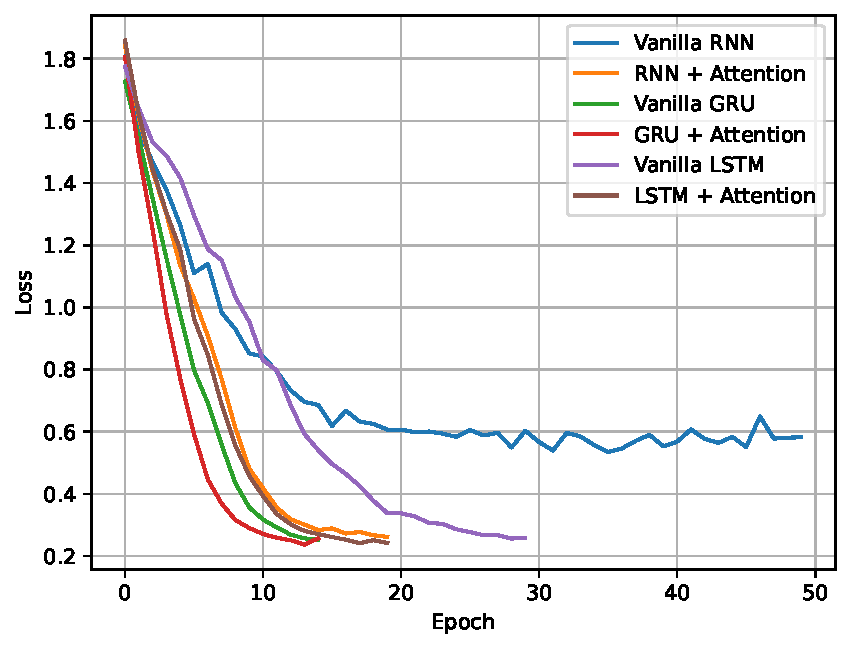
\includegraphics[width=0.9\linewidth]{./figures/vanilla.pdf}
	\caption{Epoch/Loss for from-scratch implementation}
	\label{fig:loss1}
\end{figure}

As we can observe, the vanilla RNN got stuck during the training process, which is confirmed in Table \ref{tab:tab1}. The vanilla LSTM converged to optimal weights but with poor performance, even with the attention mechanism, compared to the other models. On the other hand, the other models converged quickly and had better performance on the training set.

\begin{table}[H]
	\centering
	\begin{tabular}{@{}lccccc@{}}
		\cmidrule(l){3-6}
		\multicolumn{2}{l}{} & \multicolumn{2}{c}{Validation Set 1} & \multicolumn{2}{c}{Validation Set 2} \\ \midrule
		Model     & \#Epochs & BLEU G          & BLEU B         & BLEU G          & BLEU B         \\ \midrule
		RNN       & 50       & 0.05            & 0.02           & 0.05            & 0.02           \\
		GRU       & 15       & 0.38            & 0.35           & 0.14            & 0.12           \\
		LSTM      & 20       & 0.28            & 0.24           & 0.12            & 0.10           \\
		RNN+Att.  & 15       & 0.39            & 0.33           & 0.18            & 0.17           \\
		GRU+Att.  & 15       & 0.31            & 0.32           & 0.13            & 0.16           \\
		LSTM+Att. & 20       & 0.28            & 0.30           & 0.11            & 0.13           \\ \bottomrule
	\end{tabular}
	\caption{BLEU scores for each from-scratch model on the validation set}
	\label{tab:tab1}
\end{table}

Table \ref{tab:tab1} provides the BLEU scores for each model on two different validation sets. Validation Set 1 is the augmented dataset and Validation Set 2 is the engineering assessment only. G indicates that we used the Greedy search method to predict the translation, and B indicates beam search with width 3.

\begin{itemize}
	\item RNN: The vanilla RNN performed poorly, with BLEU scores of 0.05 and 0.02 on both validation sets, indicating that it failed to learn effectively.
	\item GRU: The GRU model showed significantly better performance, particularly on Validation Set 1, with BLEU scores of 0.38 and 0.35. However, its performance dropped on Validation Set 2.
	\item LSTM: The LSTM model performed better than the RNN but was still outperformed by the GRU and attention-based models. Its BLEU scores were 0.28 and 0.24 on Validation Set 1, and 0.12 and 0.10 on Validation Set 2.
	\item RNN+Att.: The addition of an attention mechanism to the RNN improved its performance significantly, achieving BLEU scores of 0.39 and 0.33 on Validation Set 1, and 0.18 and 0.17 on Validation Set 2.
	\item GRU+Att.: The GRU model with attention achieved slightly lower scores than the vanilla GRU on Validation Set 1 but showed a slight improvement on Validation Set 2.
	\item LSTM+Att.: The LSTM with attention had similar performance to the vanilla LSTM, indicating that the attention mechanism did not significantly improve its performance.
\end{itemize}

These result
\subsection{Fine-Tuning}
\begin{figure}[H]
	\centering
	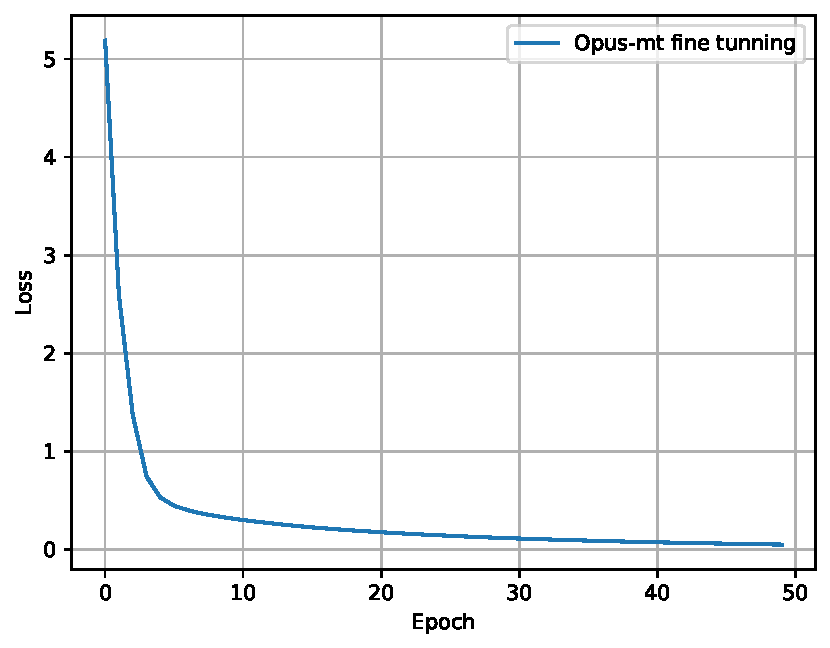
\includegraphics[width=0.9\linewidth]{./figures/fine_tunning.pdf}
	\caption{Epoch/Loss for fine-tuning implementation}
\end{figure}

\begin{table}[H]
	\centering
	\begin{tabular}{lccc}
		\toprule
		Model                 & \#Epochs & LR              & BLEU \\
		\midrule
		opus-mt-en-af         & N/A      & N/A             & 0.28 \\
		Fine-tuned opus-mt-en-af & 50      & $2\times10^{-5}$ & 0.37 \\
		\bottomrule
	\end{tabular}
	\caption{BLEU score of the original and fine-tuned opus-mt model on the validation set}
\end{table}

\subsubsection{Interpretation and Discussion}
The results from the fine-tuning experiment are shown in Figure 2 and Table 2. The original opus-mt-en-af model achieved a BLEU score of 0.28 on the validation set, whereas the fine-tuned version of the model, trained for 50 epochs with a learning rate of $2\times10^{-5}$, achieved a BLEU score of 0.37.

\begin{itemize}
	\item Original opus-mt-en-af: The pre-trained opus-mt-en-af model provided a baseline BLEU score of 0.28, indicating a reasonable performance without any fine-tuning.
	\item Fine-tuned opus-mt-en-af: The fine-tuned version of the model showed a significant improvement with a BLEU score of 0.37. This suggests that the fine-tuning process effectively adapted the pre-trained model to the specific characteristics of our dataset, improving its translation quality.
\end{itemize}

\subsubsection{Discussion of Results}
The results indicate that fine-tuning a pre-trained model can considerably enhance its performance on a specific task. The improvement in BLEU score from 0.28 to 0.37 highlights the benefits of adapting a general model to a particular domain or dataset.

Comparing the from-scratch models and the fine-tuned models, several points emerge:
\begin{itemize}
	\item Training Efficiency: The from-scratch models required careful monitoring to avoid overfitting and significant computational resources to converge. In contrast, fine-tuning a pre-trained model was more efficient and resulted in better performance.
	\item Model Performance: The best from-scratch model (RNN+Att) achieved a BLEU score of 0.39, which is close to the fine-tuned model's score of 0.37. This demonstrates that while from-scratch models can achieve competitive performance, the effort and resources required are substantially higher.
	\item Transfer Learning Benefits: The fine-tuned model's performance underscores the effectiveness of transfer learning. By leveraging a pre-trained model, we could achieve high performance with relatively fewer epochs and without extensive hyperparameter tuning.
\end{itemize}
\section{Conclusion}
In conclusion, while training models from scratch can yield high-performing models, fine-tuning pre-trained models provides a more efficient and often equally effective alternative. This approach is especially advantageous when computational resources are limited or when a quick turnaround is needed for model deployment.


\begin{thebibliography}{1}

\bibitem{kamper2022nlp817} Herman Kamper. \emph{NLP817}. \href{https://www.kamperh.com/nlp817/}{https://www.kamperh.com/nlp817/}, 2022--2024.
\bibitem{huggingface} Hugging Face \href{https://huggingface.co/}{https://huggingface.co/}
\bibitem{opus} Open Parallel Corpora \href{https://opus.nlpl.eu/}{https://opus.nlpl.eu/}
\bibitem{AdamW} AdamW \href{https://pytorch.org/docs/stable/generated/torch.optim.AdamW.html}{https://pytorch.org/docs/stable/generated/torch.optim.AdamW.html}
\bibitem{sentencepiece} Sentencepiece \href{https://github.com/google/sentencepiece}{https://github.com/google/sentencepiece}
\bibitem{helsinki} Helsinki NLP \href{https://blogs.helsinki.fi/language-technology/}{https://blogs.helsinki.fi/language-technology/}, \href{https://huggingface.co/Helsinki-NLP}{https://huggingface.co/Helsinki-NLP}
\bibitem{marian} Junczys-Dowmunt, M., Grundkiewicz, R., Dwojak, T., Hoang, H., Heafield, K., Neckermann, T., Seide, F., Germann, U., Aji, A.F., Bogoychev, N. and Martins, A.F., 2018. Marian: Fast neural machine translation in C++. \textit{arXiv preprint arXiv:1804.00344.}
\bibitem{OPUSMT} Jörg Tiedemann and Santhosh Thottingal. 2020. OPUS-MT - Building open translation services for the World. \textit{In Proceedings of the 22nd Annual Conference of the European Association for Machine Translation, pages 479–480, Lisboa, Portugal. European Association for Machine Translation.}
\end{thebibliography}